\documentclass[../main.tex]{subfiles}
\begin{document}
In this chapter, instead of installing Python 3 on your device, we can use the IDE offered by greeksforgeeks website which can be found \url{https://ide.geeksforgeeks.org/index.php}, Google Colab is a good place to write Python notebook style document. 

Python is one of the easiest advanced scripting and object-oriented programming languages to learn. Its intuitive structures and semantics are originally designed for people for are computer scientists. Python is one of the most widely used programming languages due to its:
\begin{itemize}
    \item Easy syntax and hide concept like pointers: both non-programmers and programmers can learn to code easily and at a faster rate,
    \item Readability: Python is often referred as ``executable pseudo-code'' because its syntax mostly follows the conventions used for programmers to outline their ideas.
    \item Cross-platform: Python runs on all major operating systems such as Microsoft Windows, Linux, and Mac OS X
    \item Extensible: In addition to the standard libraries there are extensive collections of freely available add-on modules, libraries, frameworks, and tool-kits. 
\end{itemize}
Compared with other programming languages, Python code is typically 3-5 times shorter than equivalent Java code, and often 5-10 times shorter than equivalent C++ code according to \url{www.python.org}. All of these simplicity and efficiency make Python an ideal language to learn under current trend, and it is also an ideal candidate language to use during Coding Interviews which is time-limited.  %However, simplicity does not necessarily perfection. Sometimes, because of Python's high level and hiding of low-level programming concepts like pointers, memory management shared by languages like C/C++ and Java can be error-prone. When immutable data types such as $list$ are passed to function directly, modifying the data structure inside of the function can lead to modification of the data structure passed in. 

% https://www.quora.com/What-is-the-difference-between-ASCII-and-unicode-characters-difference-between-UTF-8-and-UTF-16
\section{Python Overview}
\label{python_sec_overview}
In this section, we provide a well-organized overview of how Python works as an \textbf{object-oriented programming language} in Subsection~\ref{python_subsec_object}, what is the components of Python: built-in Data types, built-in modules, third party packages/libraries, frameworks (Subsection~\ref{python_subsec_components}). And in this book, we selectively introduce the most useful ones that considered for the purpose of learning algorithms and passing coding interviews.
%%%%%%understanding object%%%%%%%%%%%%%
\subsection{Understanding Objects and Operations}
\label{python_subsec_object}

\subsubsection{Basics}
\paragraph{Everything is Object} Python built-in Data Types, Modules, Classes, they are all objects. An object is a class, thus different object is just a different class. For example, we created an instance of \texttt{int} object with value \texttt{1}:
\begin{lstlisting}[language=Python]
>>> 1
1
\end{lstlisting}
We use \texttt{type()} built-in function to see its underlying type--class, for example:
\begin{lstlisting}[language=Python]
>>> type([1,2,3,4])
<class 'list'>
>>> type(1)
<class 'int'>
>>> type([1,2,3,4])
<class 'list'>
>>> type(range(10))
<class 'range'>
>>> type(1)
<class 'int'>
>>> type('abc')
<class 'str'>
\end{lstlisting}

\paragraph{Operators} Operators are used to perform operations on variables and instance of objects. The example shows operator \texttt{+} performed on two instances of objects. 
\begin{lstlisting}[language=Python]
>>> [1, 2, 3] + [4, 5, 6]
[1, 2, 3, 4, 5, 6]
\end{lstlisting}
\paragraph{Variables} When we are creating an instance of objects, a common practice is to have variables which are essentially pointers pointing to the instance of object's location in memory.
\begin{lstlisting}[language=Python]
>>> a = [1, 2, 3]
>>> b = [4, 5, 6]
>>> c = a + b
>>> c
[1, 2, 3, 4, 5, 6]
\end{lstlisting}

\paragraph{Tools} To be able to help ourselves; knowing what attributes, built-in function that, we use built-in function \texttt{dir(object)}.

To check object or function's information, we use built-in function \texttt{help}. And when we are done with viewing, type \texttt{q} to exit. 

\subsubsection{Properties}

\paragraph{In-place VS Standard Operations} In-place operation is an operation that changes directly the content of a given linear algebra, vector, matrices(Tensor) without making a copy. The operators which helps to do the operation is called in-place operator. Eg: \texttt{a+= b} is equivalent to \texttt{a= operator.iadd(a, b)}. A standard operation, on the other hand, will return a new instance of object. 

\paragraph{Mutable VS Immutable Objects} All objects can be either mutable or immutable. Simply put, for immutable data types/objects, we can not add, remove, or replace its content on the fly, whereas the mutable objects can not but rather return new objects when attempting to update.  Custom classes are generally mutable. The different behavior of mutable and immutable objects can be shown by using operations. A in-place operation can only be performed on mutable objects. 

\paragraph{Object, Type, Identity, Value}
Everything in Python is an object including different data types, modules, classes, and functions.  Each object in Python has a \textbf{type}, a \textbf{value}, and an \textbf{identity}.  When we are creating an instance of an object such as string with value `abc' it automatically comes with an ``identifier''. The identifier of the object acts as a pointer to the object's location in memory. The built-in function \texttt{id()} can be used to return the identity of an object as an integer which usually corresponds to the object's location in memory. \texttt{is} identity operator can be used directly to compare the identity of two objects. The built-in function \texttt{type()} can return the type of an object and operator \texttt{==} can be used to see if two objects has the same value.

\subsubsection{Examples}
\paragraph{Behavior of Mutable Objects}
Let us see an example, we create three variables/instances \texttt{a, b, c}, and \texttt{a, b} are assigned with object of the same value, and \texttt{c} is assigned with variable \texttt{a}.
\begin{lstlisting}[language=Python]
>>> a = [1, 2, 3]
>>> b = [1, 2, 3]
>>> c = a
>>> id(a), id(b), id(c)
(140222162413704, 140222017592328, 140222162413704)
\end{lstlisting}
We use our introduced function and operators to demonstrate its behavior. First, check \texttt{a} and \texttt{b}:
\begin{lstlisting}[language=Python]
>>> a == b, a is b, type(a) is type(b)
(True, False, True)
\end{lstlisting}
We see that \texttt{a} and \texttt{b} are having different identity, meaning the object of each points to different location in memory, they are indeed two independent objects. Now, let us compare \texttt{a} and \texttt{c} the same way:
\begin{lstlisting}[language=Python]
>>> a == c, a is c, type(a) is type(c)
(True, True, True)
\end{lstlisting}
Ta-daa! They have the same identity, meaning they point to the same piece of memory and \texttt{c} is more like an alias to \texttt{a}. Now, let's change a value in \texttt{a} use in-place operation and see its ids:
\begin{lstlisting}[language=Python]
>>> a[2] = 4
>>> id(a), id(b), id(c)
(140222162413704, 140222017592328, 140222162413704)
>>> a += [5]
>>> id(a), id(b), id(c)
(140222162413704, 140222017592328, 140222162413704)
\end{lstlisting}
We do not see any change about identity but change of values. Now, let us use other standard operations and see the behavior:
\begin{lstlisting}[language=Python]
>>> a = a + [5]
>>> a
[1, 2, 4, 5, 5]
>>> id(a), id(b), id(c)
(140222017592392, 140222017592328, 140222162413704)
\end{lstlisting}
Now, we see \texttt{a} has a different \texttt{id} compared with \texttt{c}, meaning they are no longer the same instance of the same object any more.

\paragraph{Behavior of Immutable Objects} For the mutable objects, we see the the reassignment of \texttt{c} to \texttt{a} results having same identity, however, this is not the case in the immutable objects, see an example:
\begin{lstlisting}[language=Python]
>>> a = 'abc'
>>> b = 'abc'
>>> c = a
>>> id(a), id(b), id(c)
(140222162341424, 140222162341424, 140222162341424)
\end{lstlisting}
These three variables \texttt{a, b, c} all share the same identity, meaning they all point to the same instance of object in the same piece of memory. This ends up more efficient usage of memory. Now, let's try to change the value of the variable \texttt{a}. We called \texttt{+=} operator which is  in-place operator for mutable objects:
\begin{lstlisting}[language=Python]
>>> a += 'd'
>>> a
'abcd'
>>> id(a), id(b), id(c)
(140222017638952, 140222162341424, 140222162341424)
\end{lstlisting}
We see still a new instance of string object is created and with an new id \texttt{140222017638952}.

%%%%%%%%%%%%%%%%%%%Components%%%%%%%%%%
\subsection{Python Components}
\label{python_subsec_components}
The plethora of built-in data types, built-in modules, third party modules or package/libraries, and frameworks contributes to the popularity and efficiency of coding in Python. 

\paragraph{Python Data Types} Python contains 12 built-in data types. These include four scalar data types( \textbf{int}, \textbf{float}, \textbf{complex} and \textbf{bool}), four sequence types(\textbf{string}, \textbf{list}, \textbf{tuple} and \textbf{range}), one mapping type(\textbf{dict}) and two set types(\textbf{set} and \textbf{frozenset}).  All the four scalar data types together with string, tuple, range and fronzenset are immutable, and the others are mutable. Each of these can be manipulated using:
\begin{itemize}
    \item Operators
    \item Functions
    \item Data-type methods
\end{itemize}

\textbf{Module} is a file which contains python functions, global variables etc. It is nothing but .py file which has python executable code / statement. With the build-in modules, we do not need to install external packages or include these .py files explicitly in our Python project, all we need to do is importing them directly and use their objects and corresponding methods. For example, we use built-in module Array:
\begin{lstlisting}[language=Python]
import Array
# use it
\end{lstlisting}
We can also write a .py file ourselves and import them. We provide reference to some of the popular and useful built-in modules  that is not covered in Part~\ref{part_data_structure} in Python in Section~\ref{python_sec_supplemental_tools} of this chapter, they are:
\begin{itemize}
    \item Re
\end{itemize}


\paragraph{Package/Library} Package or library is namespace which contains multiple package/modules. It is a directory which contains a special file \_\_init\_\_.py

Let’s create a directory user. Now this package contains multiple packages / modules to handle user related requests.
\begin{lstlisting}[numbers=none]
    user/      # top level package
       __init__.py
     
       get/    # first subpackage
          __init__.py
          info.py
          points.py
          transactions.py
     
      create/   # second subpackage
          __init__.py
          api.py
          platform.py

\end{lstlisting}

Now you can import it in following way
\begin{lstlisting}[language=Python]
from user.get import info # imports info module from get package
from user.create import api #imports api module from create package 
\end{lstlisting}

When we import any package, python interpreter searches for sub directories / packages.

Library is collection of various packages. There is no difference between package and python library conceptually. Have a look at requests/requests library. We use it as a package.

\paragraph{Framework} It is a collection of various libraries which architects the code flow. Let’s take example of Django which has various in-built libraries like Auth, user, database connector etc. Also, in artifical intelligence filed, we have TensorFlow, PyTorch, SkLearn framework to use. 


%%%%%%%%%%%%%%%%%%%%%%%%%%%%%%%%%%%%%%%%%%%%%%%%%%%%%%%%%%%%%%%%%%%%%%%%%%%%%%%%
% Mutable Vs Immutable
%%%%%%%%%%%%%%%%%%%%%%%%%%%%%%%%%%%%%%%%%%%%%%%%%%%%%%%%%%%%%%%%%%%%%%%%%%%%%%%%%%%
% \section{Mutable Vs Immutable}
% Not all python objects handle changes the same way. Some objects are mutable, meaning they can be altered.  Others are immutable; they cannot be changed but rather return new objects when attempting to update. What does this mean when writing python code?

% This post will talk about (a) the mutability of common data types and (b) instances where mutability matters.

% \subsubsection{Mutability of Common Types}
% The following are some immutable objects: basic scalar data types include: int, float, decimal, complex, bool, bytes. Plus the following container types
% \begin{itemize}
% \item string
% \item tuple
% \item range, what is the type of range??
% \item frozenset; which is an immutable version of set
% \end{itemize}
% The following are some mutable objects which are mostly container types:
% \begin{itemize}
% \item list
% \item dict
% \item set
% \item bytearray
% \item user-defined classes (unless specifically made immutable)
% \end{itemize}
% Because strings are immutable; what if you want to do some in-place modifications like character swapping? Use a bytearray.



\subsubsection{When Mutability Matters}
Mutability might seem like an innocuous topic, but when writing an efficient program it is essential to understand. For instance, the following code is a straightforward solution to concatenate a string together:
\begin{lstlisting}[language = Python]
string_build = ""
for data in container:
    string_build += str(data)
\end{lstlisting}
In reality, this is very \textit{inefficient}. Because strings are immutable, concatenating two strings together actually creates a third string which is the combination of the previous two. If you are iterating a lot and building a large string, you will waste a lot of memory creating and throwing away objects. Also, at the end of the iteration you will be allocating and throwing away very large string objects which is even more costly.

The following is a more efficient and pythonic way:
\begin{lstlisting}[language = Python]
builder_list = []
for data in container:
    builder_list.append(str(data))
"".join(builder_list)
 
### Another way is to use a list comprehension
"".join([str(data) for data in container])
 
### or use the map function
"".join(map(str, container))
\end{lstlisting}
This code takes advantage of the mutability of a single list object to gather your data together and then allocate a single result string to put your data in. That cuts down on the total number of objects allocated by almost half.

Another pitfall related to mutability is the following scenario:
\begin{lstlisting}[language = Python]
def my_function(param=[]):
    param.append("thing")
    return param
 
my_function() # returns ["thing"]
my_function() # returns ["thing", "thing"]
\end{lstlisting}

What you might think would happen is that by giving an empty list as a default value to param, a new empty list is allocated each time the function is called and no list is passed in. But what actually happens is that every call that uses the default list will be using the same list.  This is because Python (a) only evaluates functions definitions once, (b) evaluates default arguments as part of the function definition, and (c) allocates one mutable list for every call of that function.

Do not put a mutable object as the default value of a function parameter. Immutable types are perfectly safe. If you want to get the intended effect, do this instead:
\begin{lstlisting}[language = Python]
def my_function2(param=None):
    if param is None:
        param = []
    param.append("thing")
    return param
Conclusion
\end{lstlisting}

Mutability matters. Learn it. Primitive-like types are probably immutable. Container-like types are probably mutable.
%%%%%%%%%%%%Operators%%%%%%%%%%
\section{Data Types and Operators}

Operators are special symbols in Python that carry out arithmetic or logical computation. The value that the operator operates on is called the operand. Python offers  Arithmetic operators, Assignment Operator, Comparison Operators, Logical Operators, Bitwise Operators (shown in Chapter~\ref{chapter_bit}), and two special operators like the identity operator or the membership operator. 
\subsection{Arithmetic Operators}
Arithmetic operators are used to perform mathematical operations like addition, subtraction, multiplication etc. 
\begin{table}[h]
\begin{small}
\centering
\noindent\captionof{table}{Arithmetic operators in Python}
 \noindent \begin{tabular}{|p{0.25\columnwidth}|p{0.45\columnwidth}| p{0.20\columnwidth}| }
  \hline
Operator& Description & Example  \\ \hline

+ &	Add two operands or unary plus & 	x + y+2\\ \hline
- &	Subtract right operand from the left or unary minus  &	x - y -2\\ \hline
* 	& Multiply two operands  &	x * y\\ \hline
/ 	& Divide left operand by the right one (always results into float) &	x / y \\ \hline
% 	Modulus - remainder of the division of left operand by the right 	x % y (remainder of x/y)
// &	Floor division - division that results into whole number adjusted to the left in the number line  &	x // y \\ \hline
** &	Exponent - left operand raised to the power of right &	x**y (x to the power y)\\ \hline
\%  & Modulus - Divides left hand operand by right hand operand and returns remainder & x\% y
\end{tabular}
  \label{tab:arithematic_operators}
  \end{small}
\end{table}

\subsection{Assignment Operators}
Assignment operators are used in Python to assign values to variables.

a = 5 is a simple assignment operator that assigns the value 5 on the right to the variable a on the left.

There are various compound operators that follows the order: variable\_name (arithemetic operator) = variable or data type.  Such as a += 5 that adds to the variable and later assigns the same. It is equivalent to a = a + 5.

\subsection{Comparison Operators} 
Comparison operators are used to compare values. It either returns True or False according to the condition. 
\begin{table}[h]
\begin{small}
\centering
\noindent\captionof{table}{Comparison operators in Python}
 \noindent \begin{tabular}{|p{0.25\columnwidth}|p{0.45\columnwidth}| p{0.20\columnwidth}| }
  \hline
Operator& Description & Example  \\ \hline
> & 	Greater that - True if left operand is greater than the right &	x > y\\ \hline
< &	Less that - True if left operand is less than the right &	x < y\\ \hline
== 	& Equal to - True if both operands are equal &	x == y\\ \hline
!= &	Not equal to - True if operands are not equal &	x != y\\ \hline
>= 	& Greater than or equal to - True if left operand is greater than or equal to the right &	x >= y\\ \hline
<= 	& Less than or equal to - True if left operand is less than or equal to the right 	& x <= y\\ \hline
\end{tabular}
  \label{tab:comparison_operators}
  \end{small}
\end{table} 
\subsection{Logical Operators} 
Logical operators are the $and$, $or$, $not$ operators. It is important for us to understand what are the values that Python considers False and True. The following values are considered False, and all the other values are considered $True$. 
\begin{itemize}
    \item The $None$ type
    \item Boolean False
    \item An integer, float, or complex zero
    \item An empty sequence or mapping data type
    \item An instance of a user-defined class that defines a \_\_len\_\_() or \_\_bool\_\_() method that returns zero or False.
\end{itemize}
\begin{table}[h]
\begin{small}
\centering
\noindent\captionof{table}{Logical operators in Python}
 \noindent \begin{tabular}{|p{0.25\columnwidth}|p{0.45\columnwidth}| p{0.20\columnwidth}| }
  \hline
Operator& Description & Example  \\ \hline
and &	True if both the operands are true &	x and y\\ \hline
or &	True if either of the operands is true &	x or y\\ \hline
not &	True if operand is false (complements the operand) &	not x \\ \hline
\end{tabular}
  \label{tab:logical_operators}
  \end{small}
\end{table} 
\subsection{Special Operators}
Python language offers some special type of operators like the identity operator or the membership operator. 

\paragraph{Identity operators} Identity operators are used to check if two values (or variables) are located on the same part of the memory. Two variables that are equal does not imply that they are identical as we have shown in the last section.
\begin{table}[h]
\begin{small}
\centering
\noindent\captionof{table}{Identity operators in Python}
 \noindent \begin{tabular}{|p{0.25\columnwidth}|p{0.45\columnwidth}| p{0.20\columnwidth}| }
  \hline
Operator& Description & Example  \\ \hline
is &	True if the operands are identical (refer to the same object) &	x is y\\ \hline
is not 	& True if the operands are not identical (do not refer to the same object) & x is not y \\ \hline
\end{tabular}
  \label{tab:identity_operators}
  \end{small}
\end{table} 

\paragraph{Membership Operators}
$in$ and $not in$ are the membership operators in Python. They are used to test whether a value or variable is found in a sequence (string, list, tuple, set and dictionary).
\begin{table}[h]
\begin{small}
\centering
\noindent\captionof{table}{Membership operators in Python}
 \noindent \begin{tabular}{|p{0.25\columnwidth}|p{0.45\columnwidth}| p{0.20\columnwidth}| }
  \hline
Operator& Description & Example  \\ \hline
in &	True if value/variable is found in the sequence &	5 in x\\ \hline
not in 	& True if value/variable is not found in the sequence &	5 not in x \\ \hline
\end{tabular}
  \label{tab:membership_operators}
  \end{small}
\end{table} 

% Identity operators in Python Operator 	Meaning 	Example

% check out this link to rewrite this section. 
% % https://docs.python.org/3/library/stdtypes.html
% This section covers the various built-in operators, which Python has to offer. Having a deeper understanding of the operators can help us choose the right operator. 
% \begin{lstlisting}[numbers=none]
% Operator  Description                     Example
% +, -      Addition, Subtraction            10-3
% *, %      Multiplication, Modulo with reminder  27%7=6
% /         Division                         10/3
% //       Truncation Division (also known as floordivision or floor division)
% ~x      Bitwise negation              ~3 - 4, Result: -8 
% **      Exponentiation               10 ** 3, Result: 1000 
% or, and, not  Boolean Or, Boolean And, Boolean Not
% in      "Element of"                 1 in [3, 2, 1] 
% <, <=, >, >=, !=, ==   The usual comparison operators 
% |, &, ^   Bitwise Or, Bitwise And, Bitwise XOR
% <<, >>    Shift Operators
% \end{lstlisting}
% \textbf{Division} This operator results in different results for Python 2.x (floor division) and Python 3.x (always float). For example:
% \begin{lstlisting}[language=Python]
% # Python 3:
% 10 / 3
% # output
% # 3.3333333333333335

% #Python 2.x:
% # output 
% # 3
% \end{lstlisting}
% \textbf{Truncation Division} The result of this division is the integral part of the result, i.e. the fractional part is truncated, if there is any. It works both for integers and floating-point numbers, but there is a difference in the type of the results: If both the divident and the divisor are integers, the result will be also an integer. If either the divident or the divisor is a float, the result will be the truncated result as a float. For example:
% \begin{lstlisting}[language=Python]
% 10 // 3
% 10.0 // 3
% # output
% # 3
% # 3.0
% \end{lstlisting}
% A note about efficiency: The results of int(10 / 3) and 10 // 3 are equal. But the "//" division is more than two times as fast! 
%%%%%%%%%%%%%%%%%%%%%%%%%%%%%%%%%%%%%%%%%%%%%%%%%%%%%%%%%%%%%%%%%%%%%%%%%%%%%%%%
% Function
%%%%%%%%%%%%%%%%%%%%%%%%%%%%%%%%%%%%%%%%%%%%%%%%%%%%%%%%%%%%%%%%%%%%%%%%%%%%%%%%%%%
\section{Function}
\subsection{Python Built-in Functions}
Check out here \url{https://docs.python.org/3/library/functions.html}.
\paragraph{Built-in Data Types}
We have functions like int(), float(), str(), tuple(), list(), set(), dict(), bool(), chr(), ord(). These functions can be used for intialization, and also used for type conversion between different data types. 

\subsection{Lambda Function}
In Python, \textit{lambda function} is anonymous function, which is a function that is defined without a name. While normal functions are defined using the $def$ keyword, in anonymous functions are defined using the $lambda$ keyword, this is where the name comes from.

\paragraph{Syntax} The syntax of lambda function in Python is:
\begin{lstlisting}[language=Python]
lambda arguments: expression
\end{lstlisting}
Lambda function can has zero to multiple arguments but only one expression, which will be evaluated and returned.  For example, we define a lambda function which takes one argument $x$ and return $x^2$.
\begin{lstlisting}[language=Python]
square1 = lambda x: x**2
\end{lstlisting}

The above lambda function is equal to a normal function defined as:
\begin{lstlisting}[language=Python]
def square(x):
    return x**2
\end{lstlisting}
Calling the following code has the same output:
\begin{lstlisting}[language=Python]
square1(5) ==  square(5)
\end{lstlisting}

\paragraph{Applications} 

Hence, anonymous functions are also called lambda functions. The use of lambda creates an anonymous function (which is callable). In the case of sorted the callable only takes one parameters. Python's lambda is pretty simple. It can only do and return one thing really.

The syntax of lambda is the word lambda followed by the list of parameter names then a single block of code. The parameter list and code block are delineated by colon. This is similar to other constructs in python as well such as while, for, if and so on. They are all statements that typically have a code block. Lambda is just another instance of a statement with a code block.

We can compare the use of lambda with that of def to create a function.
\begin{lstlisting}[language = Python]
adder_lambda = lambda parameter1,parameter2: parameter1+parameter2
\end{lstlisting}
The above code equals to the following:
\begin{lstlisting}[language = Python]
def adder_regular(parameter1, parameter2): 
    return parameter1+parameter2
\end{lstlisting}



\subsection{Map, Filter and Reduce}

These are three functions which facilitate a functional approach to programming. We will discuss them one by one and understand their use cases.
\subsubsection{Map}
Map applies a function to all the items in an input\_list. Here is the blueprint:
\begin{lstlisting}[language=Python]
map(function_to_apply, list_of_inputs)
\end{lstlisting}

Most of the times we want to pass all the list elements to a function one-by-one and then collect the output. For instance:
\begin{lstlisting}[language=Python]
items = [1, 2, 3, 4, 5]
squared = []
for i in items:
    squared.append(i**2)
\end{lstlisting}
Map allows us to implement this in a much simpler and nicer way. Here you go:
\begin{lstlisting}[language=Python]
items = [1, 2, 3, 4, 5]
squared = list(map(lambda x: x**2, items))
\end{lstlisting}
Most of the times we use lambdas with map so I did the same. Instead of a list of inputs we can even have a list of functions! Here we use $x(i)$ to call the function, where $x$ is replaced with each function in funcs, and i is the input to the function.
\begin{lstlisting}[language=Python]
def multiply(x):
    return (x*x)
def add(x):
    return (x+x)

funcs = [multiply, add]
for i in range(5):
    value = list(map(lambda x: x(i), funcs))
    print(value)

# Output:
# [0, 0]
# [1, 2]
# [4, 4]
# [9, 6]
# [16, 8]
\end{lstlisting}
\subsubsection{Filter}

As the name suggests, filter creates a list of elements for which a function returns true. Here is a short and concise example:
\begin{lstlisting}[language=Python]
number_list = range(-5, 5)
less_than_zero = list(filter(lambda x: x < 0, number_list))
print(less_than_zero)

# Output: [-5, -4, -3, -2, -1]
\end{lstlisting}
The filter resembles a for loop but it is a builtin function and faster.

Note: If map and filter do not appear beautiful to you then you can read about list/dict/tuple comprehensions.
\subsubsection{Reduce}

Reduce is a really useful function for performing some computation on a list and returning the result. It applies a rolling computation to sequential pairs of values in a list. For example, if you wanted to compute the product of a list of integers.

So the normal way you might go about doing this task in python is using a basic for loop:
\begin{lstlisting}[language=Python]
product = 1
list = [1, 2, 3, 4]
for num in list:
    product = product * num

# product = 24

\end{lstlisting}
Now let’s try it with reduce:
\begin{lstlisting}[language=Python]
from functools import reduce
product = reduce((lambda x, y: x * y), [1, 2, 3, 4])

# Output: 24
\end{lstlisting}
%%%%%%%%%%%%%%%%%%%%%%%%Class %%%%%%%%%%%%%%%%%%%%%%
\section{Class}
\subsection{Special Methods}
From ~\cite{beazley2009python}. \url{http://www.informit.com/articles/article.aspx?p=453682&seqNum=6} All the built-in data types implement a collection of special object methods. The names of special methods are always preceded and followed by double underscores (\_\_). These methods are automatically triggered by the interpreter as a program executes. For example, the operation x + y is mapped to an internal method, x.\_\_add\_\_(y), and an indexing operation, x[k], is mapped to x.\_\_getitem\_\_(k). The behavior of each data type depends entirely on the set of special methods that it implements.

User-defined classes can define new objects that behave like the built-in types simply by supplying an appropriate subset of the special methods described in this section. In addition, built-in types such as lists and dictionaries can be specialized (via inheritance) by redefining some of the special methods. In this book, we only list the essential ones so that it speeds up our interview preparation. 
\paragraph{Object Creation, Destruction, and Representation} We first list these special methods in Table~\ref{tab:special_methods_for_object_creation}.
\begin{table}[h]
\begin{small}
\centering
\noindent\captionof{table}{ Special Methods for Object Creation, Destruction, and Representation}
 \noindent \begin{tabular}{|p{0.25\columnwidth}|p{0.75\columnwidth}|}
  \hline
Method& Description \\ \hline
*\_\_init\_\_(self [,*args [,**kwargs]]) &	Called to initialize a new instance\\ \hline
\_\_del\_\_(self) 	& Called to destroy an instance \\ \hline
*\_\_repr\_\_(self) & Creates a full string representation of an object \\ \hline
\_\_str\_\_(self) & Creates an informal string representation \\\hline
\_\_cmp\_\_(self,other) & Compares two objects and returns negative, zero, or positive \\\hline
\_\_hash\_\_(self) & Computes a 32-bit hash index \\hline
\_\_nonzero\_\_(self) & Returns 0 or 1 for truth-value testing \\\hline
\_\_unicode\_\_(self) & Creates a Unicode string representation \\\hline
\end{tabular}
  \label{tab:special_methods_for_object_creation}
  \end{small}
\end{table} 
A good and useful way to implement a class is through \_\_repr\_\_() method. By calling built-in function repr(built-in object) and implement self-defined class as the same as built-in object. Doing so avoids us implementing a lot of other special methods for our class and still has most of behaviors needed. For example, we define a Student class and represent it as of a tuple:
\begin{lstlisting}
class Student:
    def __init__(self, name, grade, age):
        self.name = name
        self.grade = grade
        self.age = age
    def __repr__(self):
        return repr((self.name, self.grade, self.age))
a =Student('John', 'A', 14)
print(hash(a))
print(a)
\end{lstlisting}
If we have no \_\_repr\_\_(), the output for the following test cases are:
\begin{lstlisting}[language=Python]
8766662474223
<__main__.Student object at 0x7f925cd79ef0>
\end{lstlisting}
Doing so, we has \_\_hash\_\_(), 
\paragraph{Comparison Operations} Table~\ref{tab:special_methods_for_comparison_operations} lists all the comparison methods that might need to be implemented in a class in order to apply comparison in applications such as sorting. 

\begin{table}[h]
\begin{small}
\centering
\noindent\captionof{table}{ Special Methods for Object Creation, Destruction, and Representation}
 \noindent \begin{tabular}{|p{0.25\columnwidth}|p{0.75\columnwidth}|}
  \hline
Method& Description \\ \hline
\_\_lt\_\_(self,other) & self < other \\ \hline
\_\_le\_\_(self,other) & self <= other \\ \hline
\_\_gt\_\_(self,other) & self > other  \\ \hline
\_\_ge\_\_(self,other) & self >= other  \\ \hline
\_\_eq\_\_(self,other) & self == other  \\ \hline
\_\_ne\_\_(self,other) & self != other  \\ \hline
\end{tabular}
  \label{tab:special_methods_for_comparison_operations}
  \end{small}
\end{table} 


\subsection{Class Syntax}
\subsection{Nested Class}
When we solving problem on leetcode, sometimes we need to wrap another class object inside of the solution class. We can do this with the nested class. When we re newing an instance, we use mainClassName.NestedClassName().

%%%%%%%%%%%%%%%%%%%%%%%%%%%%%%%%%%%%%%%%%%%%%%%%%%%%%%%%%%%%%%%%%%%%%%%%%%%%%%%%
% Shallow Copy and the deep copy
%%%%%%%%%%%%%%%%%%%%%%%%%%%%%%%%%%%%%%%%%%%%%%%%%%%%%%%%%%%%%%%%%%%%%%%%%%%%%%%%%%%
\section{Shallow Copy and the deep copy}
\label{shallow_deep_copy}
For list and string data structures, we constantly met the case that we need to copy. However, in programming language like C++, Python, we need to know the difference between shallow copy and deep copy. Here we only introduce the Python version. 

Given the following two snippets of Python code:
\begin{lstlisting}[language = Python]
colours1 = ["red", "green"]
colours2 = colours1
colours2 = ["rouge", "vert"]
print(colours1)
>>> ['red', 'green']
\end{lstlisting}

\begin{lstlisting}[language = Python]
colours1 = ["red", "green"]
colours2 = colours1
colours2[1] = "blue"
print(colours1)
['red', 'blue']
\end{lstlisting}

From the above outputs, we can see that the colors1 list is the same but in the second case, it is changed although we are assigning value to colors2. The result can be either wanted or not wanted. In python, to assign one list to other directly is similar to a pointer in C++, which both point to the same physical address. In the first case, colors2 is reassigned a new list, which has an new address, so now colors2 points to the address of this new list instead, which leaves the values of colors2 untouched at all. We can visualize this process as follows:
\begin{figure}[h]
\begin{subfigure}[b]{0.5\linewidth}
\centering
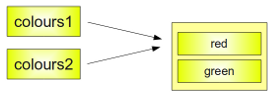
\includegraphics[width = 0.98\linewidth]{fig/deep_copy_1.png}
\caption{The copy process for code 1}
\end{subfigure}
\begin{subfigure}[b]{0.5\linewidth}
\centering
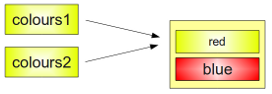
\includegraphics[width = 0.98\linewidth]{fig/deep_copy_2.png}
\caption{The copy process for code 2}
\end{subfigure}
\caption{Copy process}
\label{fig:copy_shallow}
\end{figure}
However, we often need to do copy and leave the original list or string unchanged. Because there are a variety of list, from one dimensional, two-dimensional to multi-dimensional. 
%%%%%%%%%%%%%%%%%%%%%%%%%%%%%%%%%%%%%%%%%%%%%%%%%%%%%%%%%%%%%%%%%%%%%%%%%%%%%%%%
% Shallow Copy 
%%%%%%%%%%%%%%%%%%%%%%%%%%%%%%%%%%%%%%%%%%%%%%%%%%%%%%%%%%%%%%%%%%%%%%%%%%%%%%%%%%%
\subsection{Shallow Copy using Slice Operator}
It's possible to completely copy shallow list structures with the slice operator without having any of the side effects, which we have described above:
\begin{lstlisting}[language = Python]
list1 = ['a','b','c','d']
list2 = list1[:]
list2[1] = 'x'
print(list2)
['a', 'x', 'c', 'd']
print(list1)
['a', 'b', 'c', 'd']
\end{lstlisting}
Also, for Python 3, we can use list.copy() method
\begin{lstlisting}[language = Python]
list2 = list1.copy()
\end{lstlisting}

But as soon as a list contains sublists, we have the same difficulty, i.e. just pointers to the sublists.
\begin{lstlisting}[language = Python]
lst1 = ['a','b',['ab','ba']]
lst2 = lst1[:]
\end{lstlisting}

This behaviour is depicted in the following diagram: 
\begin{figure}[h]
    \centering
    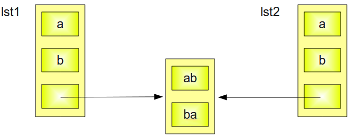
\includegraphics{fig/deep_copy_3.png}
    \caption{Caption}
    \label{fig:copy_3}
\end{figure}

If you assign a new value to the 0th Element of one of the two lists, there will be no side effect. Problems arise, if you change one of the elements of the sublist.
\begin{lstlisting}[language = Python]
>>> lst1 = ['a','b',['ab','ba']]
>>> lst2 = lst1[:]
>>> lst2[0] = 'c'
>>> lst2[2][1] = 'd'
>>> print(lst1)
['a', 'b', ['ab', 'd']]
\end{lstlisting}


The following diagram depicts what happens, if one of the elements of a sublist will be changed: Both the content of lst1 and lst2 are changed.
\begin{figure}[h]
    \centering
    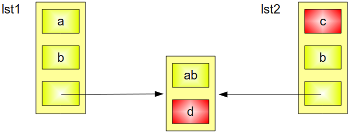
\includegraphics{fig/deep_copy_4.png}
    \caption{Caption}
    \label{fig:copy_4}
\end{figure}
\subsection{Iterables, Generators, and Yield}
\url{https://pythontips.com/2013/09/29/the-python-yield-keyword-explained/}. Seems like it can not yeild a list. 
%%%%%%%%%%%%%%%%%%%%%%%%%%%%%%%%%%%%%%%%%%%%%%%%%%%%%%%%%%%%%%%%%%%%%%%%%%%%%%%%
% Deep Copy 
%%%%%%%%%%%%%%%%%%%%%%%%%%%%%%%%%%%%%%%%%%%%%%%%%%%%%%%%%%%%%%%%%%%%%%%%%%%%%%%%%%%
\subsection{Deep Copy using copy Module}
A solution to the described problems is to use the module "copy". This module provides the method "copy", which allows a complete copy of a arbitrary list, i.e. shallow and other lists.

The following script uses our example above and this method:
\begin{lstlisting}[language = Python]
from copy import deepcopy

lst1 = ['a','b',['ab','ba']]

lst2 = deepcopy(lst1)

lst2[2][1] = "d"
lst2[0] = "c";

print lst2
print lst1
\end{lstlisting}
If we save this script under the name of deep\_copy.py and if we call the script with``python deep\_copy.p'', we will receive the following output:
\begin{lstlisting}[language = Python]
$ python deep_copy.py 
['c', 'b', ['ab', 'd']]
['a', 'b', ['ab', 'ba']]
\end{lstlisting}
\begin{figure}[h]
    \centering
    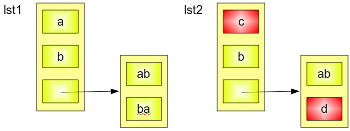
\includegraphics{fig/deep_copy_5.png}
    \caption{Caption}
    \label{fig:copy_4}
\end{figure}

This section is cited from %https://www.python-course.eu/deep_copy.php
Need to modify. 
\section{Global Vs nonlocal}

\section{Loops}
The for loop can often be needed in algorithms we have two choices: 
\textit{for} and \textit{while}. So to learn the basic grammar to do for loop easily could help us be more efficienct in programming. 

Usually for loop is used to iterate over a sequence or matrix data. For example, the following grammar works for either string or list. 
\begin{lstlisting}[language=python]
# for loop in a list to get the value directly
a = [5, 4,3, 2, 1]
for num in a:
    print(num)
# for loop in a list  use index
for idx in range(len(a)):
    print(a[idx])
# for loop in a list get both index and value directly
for idx, num in enumerate(a):
    print(idx, num)
\end{lstlisting}
Sometimes, we want to iterate two lists jointly at the same time, which requires they both have the same length. We can use \textit{zip} to join them together, and all the others for loop works just as the above. For example:
\begin{lstlisting}[language=Python]
a, b = [1, 2, 3, 4, 5], [5, 4, 3, 2, 1]
for idx, (num_a, num_b) in enumerate(zip(a, b)):
    print(idx, num_a, num_b)
\end{lstlisting}
\section{Special Skills}
\begin{enumerate}
    \item Swap the value of variable
    \begin{lstlisting}[language=Python]
    a, b = 7, 10
    print(a, b)
    a, b = b, a
    print(a, b)
    \end{lstlisting}
    \item Join all the string elements in a list to a whole string
    \begin{lstlisting}[language=Python]
    a = ["Cracking", "LeetCode, "Problems"]
    print("",join(a))
    \end{lstlisting}
    \item Find the most frequent element in a list
    \begin{lstlisting}[language=Python]
    a = [1, 3,5,6,9,9,4,10,9]
    print(max(set(a), key = a.count))
    # or use counter from the collections
    from collections import counter
    cnt = Counter(a)
    print(cnt.most_common(3))
    \end{lstlisting}
    \item Check if two strings are comprised of the same letters. 
    \begin{lstlisting}[language=Python]
    from collections import Counter
    Counter(str1) == Counter(str2)
    \end{lstlisting}
    \item Reversing
    \begin{lstlisting}[language=Python]
    # 1. reversing strings or list
    a = 'crackingleetcode'
    b = [1,2,3,4,5]
    print(a[::-1], a[::-1])
    # 2. iterate over each char of the string  or list contents in reverse order efficiently, here we use zip to 
    for char, num in zip(reversed(a), reversed(b)):
        print(char, num)
    #3. reverse each digit in an integer or float number
    num = 123456789
    print(int(str(num)[::-1]))
    \end{lstlisting}
    \item Remove the duplicates from list or string. We can convert it to set at first, but this wont keep the original order of the elements. If we want to keep the order, we can use the OrderdDict method from collections. 
    \begin{lstlisting}[language=Python]
    a = [5, 4, 4, 3, 3, 2, 1]
    no_duplicate = list(set(a))
    
    from collections import OrderedDict
    print(list(OrderedDict.fromkeys(a).keys())
    \end{lstlisting}
    \item Find the min or max element or the index. 
\end{enumerate}
%%%%%%%%%%%%%%%Supplemental Tools%%%%%%%%%
\section{Supplemental Python Tools}
\label{python_sec_supplemental_tools}
\subsection{Re}
\subsection{Bitsect}
%https://docs.python.org/2/library/bisect.html
\begin{lstlisting}[language = Python]
def index(a, x):
    'Locate the leftmost value exactly equal to x'
    i = bisect_left(a, x)
    if i != len(a) and a[i] == x:
        return i
    raise ValueError

def find_lt(a, x):
    'Find rightmost value less than x'
    i = bisect_left(a, x)
    if i:
        return a[i-1]
    raise ValueError

def find_le(a, x):
    'Find rightmost value less than or equal to x'
    i = bisect_right(a, x)
    if i:
        return a[i-1]
    raise ValueError

def find_gt(a, x):
    'Find leftmost value greater than x'
    i = bisect_right(a, x)
    if i != len(a):
        return a[i]
    raise ValueError

def find_ge(a, x):
    'Find leftmost item greater than or equal to x'
    i = bisect_left(a, x)
    if i != len(a):
        return a[i]
    raise ValueError
\end{lstlisting}

\subsection{collections}
\textbf{collections} is a module in Python that implements specialized container data types alternative to Python's general purpose built-in containers: dict, list, set, and tuple. The including container type is summarized in Table~\ref{tab:collections_container}.  Most of them we have learned in  Part \ref{part_data_structure}, therefore, in the table we simply put the reference in the table. Before we use them, we need to import each data type as:
\begin{lstlisting}[language=Python]
from collections import deque, Counter, OrderedDict, defaultdict, namedtuple
\end{lstlisting}

\begin{table}[h]
\begin{small}
\centering
\noindent\captionof{table}{ Container Data types in \textbf{collections} module.}
 \noindent \begin{tabular}{|p{0.25\columnwidth}|p{0.45\columnwidth}| p{0.20\columnwidth}| }
  \hline
Container& Description & Refer  \\ \hline
namedtuple  &  	factory function for creating tuple subclasses with named fields & \\\hline
deque  &list-like container with fast appends and pops on either end &\\ \hline
Counter  &dict subclass for counting hashable objects &\\ \hline
defaultdict  &dict subclass that calls a factory function to supply missing values & \\ \hline
OrderedDict  &dict subclass that remembers the order entries were added&\\ \hline
\end{tabular}
  \label{tab:collections_container}
  \end{small}
\end{table}
% make a table here

% %%%%%%%%%%%%%%%%%%%%%%%%%%%%%%%%%%%%%%%%%%%%%%%%%%%%%%%%%%%%%%%%%%%%%%%%%%%%%%%%
% % Exercise 
% %%%%%%%%%%%%%%%%%%%%%%%%%%%%%%%%%%%%%%%%%%%%%%%%%%%%%%%%%%%%%%%%%%%%%%%%%%%%%%%%%%%
% \section{Exercises}
% \begin{Exercise}\label{EX11} % this gives out 2.1 exercises
%         \vspace{-\baselineskip}% <-- You don't need this line of code if there's some text here
%         \Question In problem \ref{EX11-1-i}-\ref{EX11-1-iii}, determine whether the given differential equation is separable  
%         \begin{tasks}(2)
%             \task\label{EX11-1-i} $\frac{dy}{dx}-\sin{(x+y)}=0$     
%             \task $\frac{dy}{dx}=4y^2-3y+1$ 
%             \task\label{EX11-1-iii} $\frac{ds}{dt}=t\ln{(s^{2t})}+8t^2$ 
%         \end{tasks}
%         \Question In problem \ref{EX11-2-iv}-\ref{EX11-2-viii}, solve the equation 
%         \begin{tasks}[resume=true](2)
%             \task\label{EX11-2-iv} $\frac{dx}{dt}=3xt^2$
%             \task $y^{-1}dy+ye^{\cos{x}}\sin{x}dx=0$
%             \task $(x+xy^2)dx+ye^{\cos{x}}\sin{x}dx=0$
%             \task\label{EX11-2-viii} $\frac{dy}{dt} = \frac{y}{t+1} + 4t^2 +  4t$, $\quad$ $y(1) = 10$
%         \end{tasks}
% \end{Exercise}
% \setboolean{firstanswerofthechapter}{true}
%     %\begin{multicols}{2} % multicol is to make it has two cols
%         \begin{Answer}[ref={EX11}]
%             \Question 
%             \begin{tasks}
%                 \task This is a solution of Ex 1
%                 \task This is a solution of Ex 2 
%                 \task This is a solution of Ex 3 
%             \end{tasks} 
%             \Question 
%             \begin{tasks}[resume=true]
%                 \task This is a solution of Ex 4
%                 \task This is a solution of Ex 5 
%                 \task This is a solution of Ex 6 
%                 \task This is a solution of Ex 7 
%             \end{tasks} 
%         \end{Answer}
%   % \end{multicols}
% \setboolean{firstanswerofthechapter}{false}

    % \begin{Exercise}\label{EX12}
    %     Another exercise. 
    %     \Question If you don't need a horizontal list, you can simply use \verb|\Question|
    % \end{Exercise}
    % \begin{multicols}{2}
    %     \begin{Answer}[ref={EX12}]
    %         \Question This is a solution of Ex 1
    %     \end{Answer}
    % \end{multicols}


\end{document}